\documentclass[a4paper,10pt]{article}

% TODO: italic comic sans

\usepackage{ShapebyShapepréambule}

\renewcommand{\baselinestretch}{1.15}
\newcommand{\pagetitle}[2]{%
	\hspace{-0.2cm}\begin{tikzpicture}%
		\node at (-8,0) {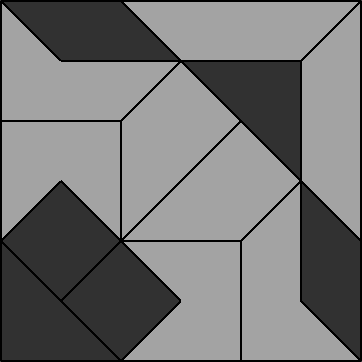
\includegraphics[width=1.5cm]{Images/Shape by shape - titre de page.png}};%
		\node at (-8,0) {\huge #1};%
		\node at (8,0) {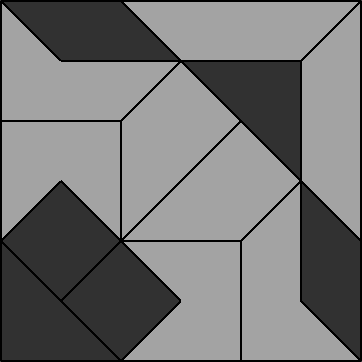
\includegraphics[width=1.5cm]{Images/Shape by shape - titre de page.png}};%
		\node at (8,0) {\huge #1};%
		%
		\node at (0,0) {\huge #2};%
	\end{tikzpicture}\vspace{1cm}%
}

\setlength{\parindent}{0pt}
\setlength{\parskip}{0.8em}

\title{Shape by shape} 
\date{}
\author{}

%%%%%%%%%%%%%%%%%%%%%%%%%%%%%%%%%%%%%%

\begin{document}


\hfill {\textbf{\LARGE APMEP - Dossier n°3131}} \hfill {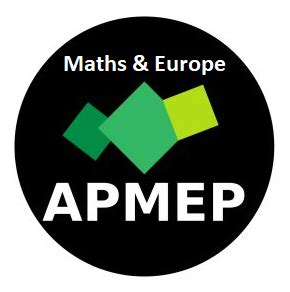
\includegraphics[width=0.15\linewidth]{Images/Shape by shape - logo AMPEP.jpeg}}

\vspace{2em}

\begin{minipage}[c]{0.45\textwidth}
	\hspace{-1.2cm}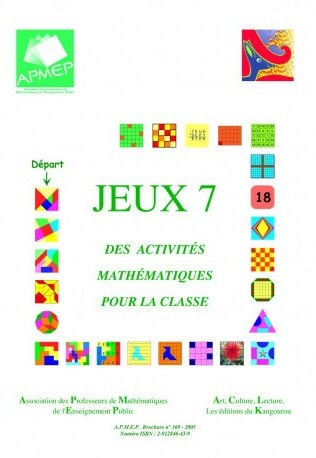
\includegraphics[width=0.8\linewidth,cframe=green 3pt,rotate=10]{Images/Shape by shape - des activités mathématiques pour la classe.jpeg}
	\vspace{1.5cm}
\end{minipage}
\begin{minipage}[c]{0.5\textwidth}
	{\Huge \textbf{Shape by Shape}}\\[1.2em]
	{\Large Activité extraite\\
	de la brochure APMEP n°169\\
	\textbf{JEUX 7} \vspace{1em}}

	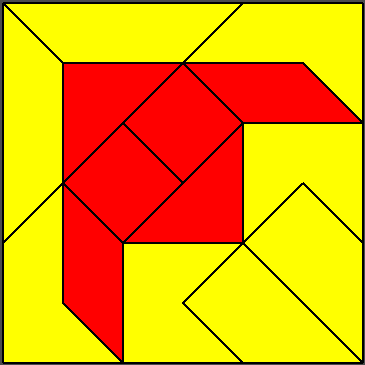
\includegraphics[width=0.5\linewidth]{Images/Shape by shape - figure 1.png} \vspace{1em}

	{\Huge Domaine : Géométrie} \\[1.5em]
	{\LARGE Cycles 3 et 4}
\end{minipage} \vspace{1em}

{
	\renewcommand{\arraystretch}{1.1}
	\Large
	\hspace{-1cm}\begin{tabular}{ll}
		Fiche 0       & Présentation                                             \\
		Fiche 1       & À la découverte d'un jeu (\textit{recherche des pièces}) \\
		Fiche 2       & De l'aire, de l'aire !                                   \\
		Fiche 3       & Périmètres en toutes lettres                             \\
		Fiche 4       & Aires et périmètres                                      \\
		Fiche 7 et 8  & Symétrie axiale                                          \\
		Fiche 9 et 10 & Symétries axiale et centrale                             \\
		Fiche 13      & Des rectangles, des aires et des périmètres              \\
	\end{tabular} \vspace{2em}
}

\hfill \textit{\Large Avec les solutions} \vspace{1em}

\begin{center}
	Association des Professeurs de Mathématiques de l'Enseignement Public

	APMEP - Brochure n°169 - 2005

	Numéro ISBN : 978-2-912846-43-9
\end{center}

\newpage

\hspace{-1.2cm}\begin{tikzpicture}
	\node at (-8,0) {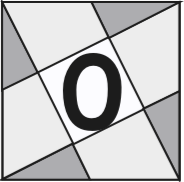
\includegraphics[width=1.5cm]{Images/Shape by shape - titre de page 0.png}};
	\node at (8,0) {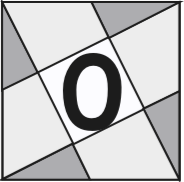
\includegraphics[width=1.5cm]{Images/Shape by shape - titre de page 0.png}};
	\node at (0,0) {\Huge PUZZLES et MATHÉMATIQUES};
\end{tikzpicture}\vspace{2cm}

\noindent {\large Shape by Shape} \\

Récemment, est apparu dans le commerce un jeu nommé « Shape by Shape », édité par « Binary Arts Compagny », utilisant deux fois les « diabolos » et les « tétrabolos ». Nous utilisons les pièces de ce jeu pour faire faire des mathématiques à nos élèves (à l'origine, les pièces du jeu sont jaunes et rouges ; pour des facilités de reprographie, nous les nommons les pièces foncées et les pièces claires).

\textbf{Aires} (page 2) : Les aires sont ici privilégiées. Des polygones autres que ceux demandés dans l'activité sont envisageables.

\textbf{Aire et périmètre} (pages 3 et 4) : Nous pouvons considérer que les pièces foncées ont une aires de mesure 2 et les pièces claires une aire de mesure 3. Les périmètres diffèrent et sont ici exprimés en fonction de deux longeurs « p » et « g ».

\textbf{Symétrie axiale et centrale (1)} (pages 7 et 9) : La reconnaissance d'éléments de symétrie pour les pièces est demandée. Les assemblages de deux pièces « identiques » par une symétrie axiale sont demandés. Le même travail est imaginé pour des symétries centrales.

\textbf{Symétrie axiale et centrale (2)} (pages 8 et 10) : Les pièces foncées peuvent être assemblées de manière symétrique. Les pièces claires auront alors à compléter le carré du plateau de jeu. Symétries orthogonales et symétries centrales sont sollicitées. La recherche de ces configurations est voisine de ce qui est proposé sur les cartes imaginées par les créateurs du jeu.

\textbf{Activités complémentaires} (page 13) : Nous proposons quelques défis utilisant les pièces du jeu et alliant périmètre, aire et écritures littérales.

\textbf{Matériel} (page 15) : Ici aussi le carton de récupération sera le bienvenu. Les collages « recto » « verso » sont prévus en respectant l'épaisseur du carton, la feuille permet la réaliqation de deux exemplaires des pièces du jeu.

Le jeu « Shape by Shape » associe deux types de pièces formées de deux ou trois triangles rectangles isocèles.

\vfill

\begin{center}
	\hspace{0.5cm}
	\LARGE
	\textit{La réussite d'une personne est déterminée par} \hspace{0.5cm}

	\hspace{0.5cm}\textit{les jeux de son enfance.} \large \hfill Tamil \hspace{0.5cm}
\end{center}

\vspace{2cm}

\hfill {\scriptsize JEUX 7 - Brochure A.P.M.E.P. n°169 - 2005} \hfill {\small 3}

\newpage

\pagetitle{1}{Shape by Shape}

\end{document}